\section{From \coco to Java}\label{sec:co2-to-java}


In \coco a service is represented as an agent $\sys{\pmv{A}}{\procP}$ that can offer (or require) some behaviour by advertising it in the form of a session type $\contrP$ (\Cref{def:co2:syntax} and \Cref{def:contracts:syntax}).

Our goal is to obtain a Java executable program with the same behaviour of the \coco agent, generating its code automatically.

In order to do so, we need first to extend the \textit{contract-oriented middleware} API (\Cref{sec:co2-middleware}) and then we need a contract model for the automated code generation (\Cref{sec:co2-plugin}) and for the verification of the honesty (\Cref{chap:java-honesty}).

%Note that we can translate only a subset of all processes permitted by \coco, as shown on \Cref{sec:untranslatable-code}.


\subsection*{Extended \coco Java API}\label{sec:extended-api}
In this section we illustrate the \textit{extended} API, which is necessary to auto-generate the code from \coco syntax (\Cref{sec:co2-plugin}) and make it analyzable by Java PathFinder (JPF, described in \Cref{chap:java-honesty}).


\subsection{Contracts}\label{sec:java-contracts-model}
The first limitation of the middleware API is how contracts are represented. As focused in \Cref{sec:co2-middleware-api}, the only way to handle contracts is building a \incodeType{String} object, describing an XML document or \textit{timed session-types} \cite{Bartoletti15forte}. Working with strings is cumbersome because we need the possibility to navigate a contract in order to verify the honesty of a process.

We removed this limit by modelling contracts as Java classes that, on interfacing with the middleware, are serialized to one of the forms explained above: the chosen \textit{target format} is  the \textit{timed session-types} because it easily includes our specification.

\begin{figure}
	\centering
	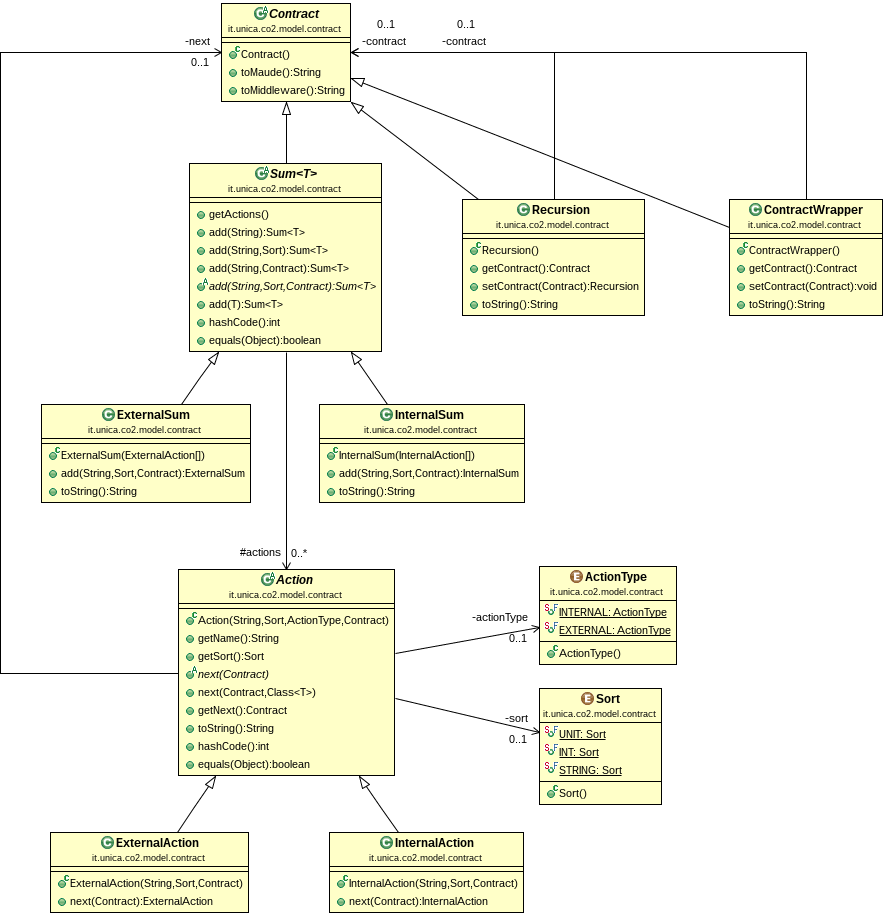
\includegraphics[scale=0.4]{img/class-diag/contracts.png}
	\caption{Class diagram of contracts}
	\label{fig:class-diag-contracts}
\end{figure}

\Cref{fig:class-diag-contracts} shows the class diagram of contracts. The \textit{abstract} class \incodeType{Contract} provides two utility methods, \incodeMethod{toMaude()} and \incodeMethod{toMiddleware()} that return the \incodeType{String} representation of the contract respectively in Maude syntax (needed for the honesty check) and timed session-types syntax (without the time guards).

\incodeType{Contract} is extended by the abstract class \incodeType{Sum}\generic[Action]{T} and the concrete classes \incodeType{Recursion} and \incodeType{ContractWrapper}. 

The \incodeType{Sum} is extended by \incodeType{ExternalSum}\generic{ExternalAction} and \incodeType{InternalSum}\generic{InternalAction}, that respectively represent the \textit{external} and \textit{internal choices} described in \Cref{def:contracts:syntax}.
The simplest way to construct a sum is shown in \Cref{lst:contract-sum}: the overloaded method \incodeType{Sum}\generic{T}.\incodeMethod{add(...)} allows to add an action \incodeType{T}, specifies its \incodeType{Sort}, and sets the next contract. %Remember that session-types (\Cref{def:contracts:syntax}) not allow to define a \textit{sequence} directly, although you can obtain it with a chain of ``single-action'' sums.
%
%\begin{listing}
%	\inputJavaLineos{code/ex-contract-sum.txt}
%	\caption{Example of contract sums.}
%	\label{lst:contract-sum}
%\end{listing}

The  \incodeType{Recursion} and \incodeType{ContractWrapper} are substantially identical but with different semantics: a \incodeType{Recursion} is used to define \textit{recursive behaviour}, while the \incodeType{ContractWrapper} was introduced as a workaround to the Java restriction that (properly) one cannot refer to a variable not yet initialized. The latter has become necessary on automated code-generation (explained in \Cref{sec:co2-plugin}). 

An example of a recursive contract is shown in \Cref{lst:contract-rec}, where \incode{R} and \incode{C} represent the same contract (if \incode{R} is expanded, we obtain \incode{C}): at line \lineno{6} we set \incode{R} as the \textit{next} contract of \incodeKeyword{a} (\incode{R} is still undefined); at line \lineno{7} we set \incode{C} as the body of \incode{R}. The contract are represented by session-types, $\contr{R} = \rec{X}{ \atomOut{a} \contrSeq X \sumInt \atomOut{b} }$ while $\contr{C} = \atomOut{a} \contrSeq \rec{X}{(\atomOut{a} \contrSeq X \sumInt \atomOut{b})} \sumInt \atomOut{b}$.
%
%\begin{listing}
%	\inputJavaLineos{code/ex-contract-rec.txt}%
%	\caption{Example of recursive contract.}
%	\label{lst:contract-rec}
%\end{listing}



\subsection{Prefixes}
\coco prefixes are modelled in Java as method calls. These methods are defined mainly into two classes, \incodeType{Session2} %\generic[ContractModel]{T}
 and \incodeType{Participant}. The former provides those prefixes that require a \textit{fused} session, \ie send/receive; the latter simplifies the advertisement of a \incodeType{Contract} and the establishment of a session with another participant.

\subsubsection{Participant}
The abstract class \incodeType{Participant} models a \coco agent $\sys{\pmv{A}}{\procP}$ and provides some methods that simplify the usage of middleware API and are necessary to analyze the code with JPF. This methods are:
%
\begin{description}
	\item[\incodeMethod{tell(\incodeType{Contract})} : \incodeType{Public}] \hfill \\
	Tells the given contract and returns a \incodeType{Public} without waiting for a session. Corresponds to the \coco prefix $\tell {} {\freeze x \contrP}$.
%
	\item[\incodeMethod{tellAndWait(\incodeType{Contract})} : \incodeType{Session2}] \hfill \\
	Tells the given contract and waits until a session is fused. Corresponds to the \coco prefix $\tell {} {\freeze x \contrP} \cocoSeq \ask{x}{true}$.
%	
	\item[\incodeMethod{waitForSession(\incodeType{Public})} : \incodeType{Session2}] \hfill \\
	Blocks the execution until a session is fused and assumes you already invoke \incodeMethod{tell(\incodeType{Contract})}. Corresponds to the \coco prefix $\ask{x}{true}$.
%	
	\item[\incodeMethod{waitForSession(\incodeType{Public},\incodeType{Integer})} : \incodeType{Session2}] \hfill \\
	As above, but specifying a timeout and throwing an exception if it expires. Corresponds to the \coco prefix $\ask{x}{true} \cocoPlus \tau$.
\end{description}

%\begin{figure}
%	\centering
%	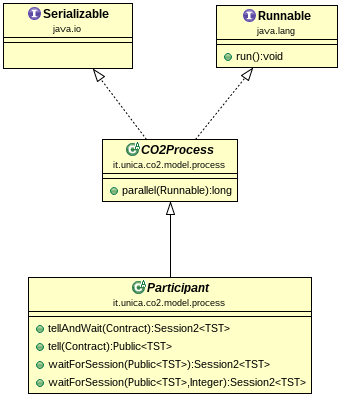
\includegraphics[scale=0.5]{img/class-diag/co2-processes.png}
%	\caption{Class diagram of precesses}
%	\label{fig:class-diag-processes}
%\end{figure}


%\begin{listing}[hp]
%	\inputJavaLineos{code/ex-process-participant.txt}
%	\caption{Example of a participant.}
%	\label{lst:process-participant}
%\end{listing}

The \incodeType{Participant} class extends the  \incodeType{CO2Process}, which implements the interfaces \incodeType{Serializable} (required by JPF) and \incodeType{Runnable}. The \incodeMethod{run()} method defines the ``behaviour'' of the process.
\Cref{lst:process-participant} shows a simple complete participant implementation.
%

\subsection{Parallel process}
\coco parallel processes are implemented as Java \incodeType{Thread}s and this explains the runnable nature of a participant. In fact the \incodeType{CO2Process} provides the following method:
%
\begin{description}
	\item[\incodeMethod{parallel(\incodeType{Runnable})} : \incodeType{long}] \hfill \\
	It starts a new \incodeType{Thread} that executes the given \incodeType{Runnable} object and returns the id of the thread.
\end{description}
%

%\begin{listing}
%	\inputJavaLineos{code/ex-process-parallel.txt}
%	\caption{Example of a parallel process.}
%	\label{lst:process-parallel}
%\end{listing}


In Java 8, you can invoke it taking advantage \textit{lambda expressions}. \Cref{lst:process-parallel} show you a process that take use of the parallel construct.


\subsection{Session}

The class \incodeType{Session} %\generic[ContractModel]{T}
(provided by the middleware API) lacks of some useful methods. A desirable method is \incodeMethod{waitForReceive(\incodeType{\incodeType{String\dots}\;\incodeBlack{actions}})} that takes as parameters the actions you want to receive: it waits until one of the specified actions is received.

Moreover, \incodeType{Session} does not provide a unique identifier, which would simplify the JPF analysis.
Therefore we extends it with the class \incodeType{Session2}, %\generic[ContractModel]{T}
whose most important methods are:
%
\begin{description}
	\item[\incodeMethod{waitForReceive(\incodeType{String\dots}\;\incodeBlack{actions})}]\label{item:session-wait} \hfill \\
	Corresponds to a sum of receive, \eg $\fact x {\atomIn{a}} \cocoPlus	\fact x {\atomIn{b}} \cocoPlus \fact x {\atomIn{c}}$.
	
	\item[\incodeMethod{waitForReceive(\incodeType{Integer} \incodeBlack{timeout,} \incodeType{String\dots}\;\incodeBlack{actions})}]\label{item:session-wait-timeout} \hfill \\
	Corresponds to a sum of receive with the timeout branch, \eg $\fact x {\atomIn{a}} \cocoPlus	\fact x {\atomIn{b}} \cocoPlus \fact x {\atomIn{c}} \cocoPlus \tau$.
	
	\item[\incodeMethod{send(\incodeType{String} \incodeBlack{action})}] \hfill \\
	This method corresponds to \coco the prefix $\fact x {\atomOut{a}}$.
	
	\item[\incodeMethod{send(\incodeType{String} \incodeBlack{action,} \incodeType{Integer} \incodeBlack{value})}] \hfill \\
	This method corresponds to \coco the prefix $\fact x {\atomOut{a}} e$ with $e$ of sort $\sort{int}$.
	
	\item[\incodeMethod{send(\incodeType{String} \incodeBlack{action,} \incodeType{String} \incodeBlack{value})}] \hfill \\
	This method corresponds to \coco the prefix $\fact x {\atomOut{a}} e$ with $e$ of sort $\sort{string}$.
	
\end{description}


%\begin{figure}
%	\centering
%	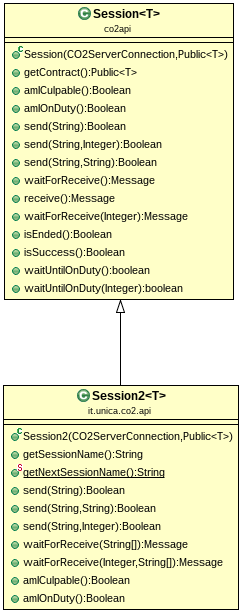
\includegraphics[scale=0.5]{img/class-diag/session2.png}
%	\caption{Class diagram of sessions}
%	\label{fig:class-diag-session2}
%\end{figure}


\subsection{Untranslatable code}\label{sec:untranslatable-code}
Not all \coco processes can be translated to Java code, due to language limits or the lack of sense. For example consider the non-deterministic choice of the sum process: the semantics (\Cref{fig:co2:semantics}) states that any prefix can be \textit{consumed} if permitted by the \textit{contract configuration}. 

In Java, we do not trace contract configuration changes, so there is no way to translate sums without losing the semantics, except for these ones that contain input prefixes (\eg $\fact x {\atomIn{a}} \cocoPlus \fact x {\atomIn{b}}$ or $\fact x {\atomIn{a}} \cocoPlus	\fact x {\atomIn{b}} \cocoPlus \tau$), in which the branch is chosen based on an external input. Even in this case, we can translate only sums of actions of the same type.
Now consider the process $\fact x {\atomOut{a}} \cocoPlus	\fact x {\atomOut{b}} \cocoPlus \fact x {\atomOut{c}}$: at first glance, you can be tempted to use the \incodeType{Random} class to make a choice and fire an output. However, this approach is not correct because the choice is made without considering the contract configuration and the corresponding \coco process would be $\tau \cocoSeq \fact x {\atomOut{a}} \cocoPlus	\tau \cocoSeq \fact x {\atomOut{b}} \cocoPlus \tau \cocoSeq \fact x {\atomOut{c}}$, whose meaning is different by the first one.

Furthermore we cannot translate processes if the $\ask{}{}$ prefix is missed before the use of a session. This limitations is now related to the fact that a session must be explicitly requested to the middleware. %For the same reason, we cannot pass a session as an actual parameter if is not preceded by an $\ask{}{}$.


\section{\coco Eclipse plugin}\label{sec:co2-plugin}

The \coco Eclipse plugin is implemented with Xtext, a framework for development of programming languages and \textit{Domain Specific Languages} (DSL) (\Cref{sec:xtext}), which moreover is part of the Eclipse ecosystem and maintained as an official project. The correct way of define our plugin would be \textit{Xtext plugin}: in fact we create an Xtext project, which provides all the scaffolding classes needed to add special functionality like code validation, syntax highlighting, etc.

\subsection{Grammar definition}

We define the \coco grammar using the Xtext DSL. Since the generated parser is LL(*), it is simple to write a grammar that fulfils the \coco specifications (although we must careful to not abuse of \textit{backtracking} due to performance reasons). The basic idea is that each rule corresponds to a Java class (instantiated when building the AST) and each declaration inside a rule is mapped to a class field. The implemented Xtext grammars are shown on \Cref{appchap:xtext-grammars}, categorized by type.

%\inputCocoFloat[h]{code/co2/sample.co2}{Example of \coco system}{lst:co2-sample}

\Cref{lst:co2-sample} is an example of a \coco process you can write with the plugin:
%
\begin{description}
	\item[\textnormal{Line \lineno{1}}] \hfill \\
	declares the system fully qualified name, used to generate \textit{target files} when the code will be translated to Maude and Java syntax.
	%
	\item[\textnormal{Line \lineno{3}}] \hfill \\
	specifies the main process that is considered for the honesty check (you can omit the whole line).
	%
	\item[\textnormal{Lines \lineno{5} and \lineno{9}}] \hfill   \\
	declare two contracts in which the former (a single-element external sum) is composed of the latter (an internal sum). Internal and external sums are respectively formed as  
	\incode{a1!} \incodeKeyword{T} \incode{+} \incode{a2!} \incodeKeyword{T}  \incode{+} \incode{aN!} \incodeKeyword{T} and 
	\incode{a1?} \incodeKeyword{T} \incode{(+)} \incode{a2?} \incodeKeyword{T}  \incode{(+)} \incode{aN?} \incodeKeyword{T}, where \incodeKeyword{T} can be \inlineCoco{int}, \inlineCoco{string} and \inlineCoco{unit} (in this case can be omitted).
	%
	\item[\textnormal{Lines \lineno{13} and \lineno{17}}] \hfill \\
	define the two processes \incode{P} and \incode{P1}.	
	Process \incode{P} declares a \textit{freename} of type \inlineCoco{session}, tell the contract \incode{C} and waits until the session \incode{y} is fused. Next, it waits for the action \incode{value}, storing the received value into the variable \incode{n} of type \inlineCoco{int}. Finally calls \incode{P1} with actual parameters \incode{n} and \incode{y}.	
	Process \incode{P1} takes the value \incode{n} and the session \incode{x}, next sends the action \incode{greater} if \incode{n>0}, \incode{lower} otherwise.
%
\end{description}

The keyword \inlineCoco{nil} defines an empty contract/process. The supported sorts are \inlineCoco{int}, \inlineCoco{string} and \inlineCoco{unit} for the declaration of actions into contracts, and \inlineCoco{int}, \inlineCoco{string}, \inlineCoco{boolean} and \inlineCoco{session} for the declaration of freenames.

\Cref{chap:use-cases} contains more complicated examples showing the completeness of the grammar.

\subsection{Scoping}
The scope of a name binding is the part of the program where the binding is valid. Xtext provides an out-of-the-box scoping system that can be customized to fit particular requirements. 

\subsubsection{Contracts}
Contracts contain two type of references, one to another contract and one to a recursion definition. The former is resolved between all contracts definition in the same file, except the one containing the reference, while the latter is resolved between all recursions defined into the same contract and \emph{before} the reference.

\Cref{lst:co2-contract-scope} shows an example of scoping. \incode{C1} is a recursive contract, \incode{C2} and \incode{C3} are two semantically equivalent contracts, but the scope of \incode{A} is limited to \incode{C1} so \incode{C2} does not compile.
Also \incode{C1} and \incode{C4} are semantically equivalent, but the visibility of \incode{C4} is hidden within \incode{C4} itself.
%
This behaviour is a little bit cumbersome and error prone: to avoid problems, you must use the \inlineCoco{rec} construct to define \textit{recursive behaviour} and use references between contracts only for \textit{composition} (manually avoiding loops). The scoping rules try to mitigate this problem, but these ones can be bypassed as shown in \Cref{lst:co2-contract-infinite}. This problem will be resolved in the future.

%\inputCocoFloat{code/co2/contracts-scope.co2}{Example of contract scoping}{lst:co2-contract-scope}

%\inputCocoFloat{code/co2/contracts-infinite.co2}{Example of infinite contract loop}{lst:co2-contract-infinite}

\subsubsection{Processes}
Processes can contain references to contracts and to other processes, allowing composition and recursive behaviour. Both contracts and processes references are resolved among all the declarations inside the same file.



\subsection{Validation}
Custom validations were added according to \coco language specification. The validation phase occurs after the parsing and linking phases, covered automatically by Xtext based on the grammar definition and the scoping customization.

The validation phase covers not only errors reporting, but warnings and info too. Consider for example if a freename declaration hides another one, maybe without changing its type: the process is correct (respecting the syntax and the static typing), but can lead to an unexpected behaviour if you do not see the freename you're hiding, so we report a warning.

Implemented validations are:
\begin{description}\itemsep0pt

	\item[\error{error}:] uniqueness of process names on declarations
	
	\item[\error{error}:] uniqueness of contract names on declarations
	
	\item[\error{error}:] the \inlineCoco{honesty} keyword must be followed by a process reference that takes no arguments

	\item[\error{error}:] action names inside a contract sums must be unique, \ie neither \inlineCoco{a! (+) a!} nor \inlineCoco{a? + a?} are permitted
	
	\item[\warning{warning}:] freenames shadowing (including recursion names)
	
	\item[\info{info}:] the \inlineCoco{unit} action type can be omitted
	
	\item[\info{info}:] the \inlineCoco{nil} keyword, representing empty contracts and  processes, can be omitted
	
\end{description}

\subsubsection{Type system}
The \coco type system is implemented using Xsemantics, a DSL (implemented in Xtext itself) for writing type systems, reduction rules, interpreters (and in general relation rules) for languages implemented in Xtext.

Into our grammar, \textit{freenames} can be declared and used in different places (see \Cref{appsec:xtext-co2} for details). The declaration of a freename can occur in a formal parameter, in a delimited process or in a input prefix: any type can be used among \inlineCoco{int}, \inlineCoco{string}, \inlineCoco{boolean} and \inlineCoco{session} when declaring a formal parameter or a delimited process, while input variables are limited to \inlineCoco{int} and \inlineCoco{string} type.

Referred freenames can be used inside an expressions, except for the \inlineCoco{session} type. Furthermore, we check the match between the actual and formal parameters types on process invocation.

%\begin{listing}
%	\inputJavaLineos{code/xtext/sample.xsemantics}
%	\caption{Part of the type-system rules}
%	\label{lst:xsemantics-sample}
%\end{listing}

Into practice, we implement a set of \textit{rules} whose result (a Java type) depends on a set of \textit{premises}. Rules without premises are \textit{axioms}. Considering this aspect, is possible to write potentially any validation rule using the Xsemantics engine. \Cref{lst:xsemantics-sample} shows some simple rules and we refer to \Cref{appsec:xsemantics} for the full implementation.


\subsection{Code generation}
The plugin can automatically transform from \coco syntax to Maude and Java languages.
The code generation happens navigating the AST and translating each \coco construct to the corresponding code of the target language. The Maude representation of \coco is complete, so it is always possible to obtain a translation and verify the honesty of the process using \cite{verifiable}, as explained in \Cref{sec:maude:checker}. On the other hand, as focused in \Cref{sec:untranslatable-code}, not all processes can be translated to Java.

The \inlineCoco{system} declaration is used to produce the target files, \eg \inlineCoco{system} \inlineCoco{com.example.co2.Sample} will produces \textit{Sample.maude} and \textit{Sample.java} inside the directory structure \texttt{/com/example/co2/Sample}.

A complete example of auto-generated code can be found in \Cref{chap:use-cases}.